\documentclass{ecscw2007}
\usepackage{graphicx}
\graphicspath{{./figures/}}

%\usepackage[romanian]{babel}
\usepackage{ucs}
\usepackage[utf8]{inputenc}


%%\usepackage{color}
%%\usepackage[pdfmark,bookmarksopen,colorlinks,urlcolor=red]{hyperref}
%%\usepackage{url}

\title{AETHER in ParaDe: Setting the Stage for Awareness Engine Experimentation}
\author{Author 1, Author 2}
\affiliation{Institute 1, Country, Institute 2, Country} 
\email{author1@institute1.org, author1@institute1.org}

%%%%%% PDF setup
%%\hypersetup{pdftitle={}}
%%\hypersetup{pdfsubject={}}
%%\hypersetup{pdfkeywords={}}
%%\hypersetup{pdfauthor={S Luz (luzs@)}}
%%\hypersetup{citecolor=red}

\pagestyle{empty}

\begin{document}

\maketitle
\thispagestyle{empty}

% TODO Şandor
% TODO anticipative awareness

\begin{abstract}
We are in the process of assembling an awareness engine experimentation ground. The AETHER awareness engine principles still look promising after more than a decade, yet their implementation and long-term use on real-life systems were hampered by a number of issues, which we describe in this paper. Due to such issues we believe that generic awareness engine support for groupware is still far in the future, and therefore it is important, as an intermediate step, to build experimentation grounds for awareness engines like AETHER. We found a suitable setting for such experimentation in a collaborative programming application called ParaDe. We implemented generic AETHER awareness support for ParaDe and we are preparing experimentation in regard to awareness widgets, awareness engine performance, awareness engine configuration, and long-term evaluation of AETHER-mediated awareness in the collaborative tool. Experimentation will involve the participation of ParaDe users.
\end{abstract}

\section*{Introduction}
Awareness has long been a topic of concern for CSCW and has developed in a large variety of ways (\cite{schmidt02}) that make it a problematic concept, yet do not reduce the considerable amount of interest. Developing frameworks for supporting awareness in a generic way within CSCW systems has come naturally within this concern, with systems such as GroupDesk (\cite{fuchs95}), BSCW (\cite{bentley97}), and Interlocus \cite{nomura98}), NESSIE (\cite{prinz99}). Most such systems come with a conceptual framework that theorizes and models awareness. Other researchers have focused on design frameworks focusing on, for example, workspace awareness (\cite{gutwin02}), and ``past events awareness'' (\cite{kirsch-pinheiro03}). A generic spatial theory of awareness ``with strong relation to physical reality and therefore [] highly intuitive nature'' was developed for virtual reality systems under the name of Spatial Model by \cite{benford93}.
%, further formalized by \cite{rodden96}
The Spatial Model has at its core the concepts of focus and nimbus; the focus represents what a user is interested in, and the nimbus of an object is meant to 'attract' user attention to it.
%An object in a virtual space carries with it an aura (a sub-space around the object) which, if it intersects the aura of another object, makes it possible for awareness to exist between the two. 
%The level of intensity to which the awareness will exist depends on focus and nimbus. 
%More precisely 
Then 
``the level of awareness that object A has of object B in Medium M is some function of A's focus in M and B's nimbus in M''.


%Collaborative Virtual Environments employ geometrical spaces, so in their early days, aura, focus and nimbus were defined as subspaces of a geometrical virtual space. Furthermore, the existence of an awareness level between A and B meant that potentially expensive (as limited resources) communication channels in medium M needed to be open, which explains the main reason for the existence of aura: it served as a filter to avoid unnecessary computation of awareness levels and unnecessary allocation of communication resources. 

% Starting from Rodden's (1996) abstract mapping of aura, focus and nimbus to non-geometrical spaces,
The AETHER model was proposed as a basic service that CSCW systems could offer, in order for their applications to benefit from generic awareness level computation between the objects these applications work with. As different from the initial Spatial Model, AETHER works in a non-geometric space called semantic network made by whatever objects the applications work with, including documents, messages, calendar and task records, etc. Aura, focus and nimbus are said to \textit{percolate} in this space. AETHER thus presents an ambitious model that aims to fulfill the needs of as many collaborative applications and systems as possible. It is also based on a strong correspondence with physical reality, so apart from its theoretical sophistications, its base on aura, focus and nimbus is of intuitive nature.
% A very computationally intensive implementation was available at the time of its proposal, yet the practical efforts in its further deployment and evaluation were hampered by a number of issues to which we turn now. 

\subsection*{Issues with Aether}
Several concerns have arisen in continuing with AETHER realization and evaluation in realistic settings. While AETHER takes good care of the percolation and matching mechanisms once focus and nimbus were established, it was not clear what would be the levers by which the user can manipulate focus and nimbus. 
%In an unfortunate case, this can be related to Grudin's (1994) concept of prisoner�s dilemma in relation to groupware, where extra user work would be needed to take care of foci and nimbi without the user benefiting directly from that work.
We will call this our \textit{focus-nimbus manipulation concern}. Practically building and maintaining such semantic networks with information extracted from off-the-shelf applications is very difficult, as these applications have closed document models. This is the \textit{semantic network buildup} concern. The concern is not only related to the availability of data for a semantic network but also to the quality of the data. Often a relation between two objects that are present in a semantic network exists in a medium or form that is not accessible to the awareness engine, thereby compromising its abilities to perform useful percolation. The complexity of processing mechanisms taking place in an Aether engine may be difficult for end users to comprehend. We take from Dourish and Button (1998) a \textit{translucency concern} that should enable artefacts we build to be sufficiently transparent for our users to be able to understand, or delve more into the details that they whish to understand, without needing to expose all technical details of the mechanisms' implementation. 
%As Dourish and Button put it
%\begin{quote}By revealing more of what lies behind them, [] 'translucent' interfaces [] provide cues as to not only what the system was doing, but why it was being done, and what was likely to be done next, uniquely for the immediate circumstances
%\end{quote}
Also related to complexity of an awareness engine, as well as to understanding its mechanisms, is the issue of configuration of such mechanisms, and share such configurations with other users. This \textit{tailoring concern} has long been pressing in CSCW, yet it was not much addressed in relation to awareness platforms. However we do not believe that such issues should prevent CSCW from experimenting further with awareness engines. Instead, they are design challenges that should be addressed. We identified ParaDe, a collaborative programming sandbox, as a suitable ground for starting to address these issues through experimentation. 

\section*{ParaDe: awareness engine experimentation field} 
ParaDe (Parallel Development, \cite{bogdan-coop08}) has been designed for a group of amateur programmers to be able to maintain the code of a large intranet of a student organization spread out in 70 locations in Europe. It has been used since 2002 by a team of volunteers which has numbered between 10 and 20 programmers, and between 5 and 10 testers. As in many student settings, membership of the team has changed quite often, yet the voluntary activity could be sustained, to develop and maintain the student organization intranet which at present consists of over 2300 source code files. The team of programmers works in a highly ad-hoc manner, without fixed times for work, with various times and  periods of engagement with the programming activity, and scattered over the 70 locations, with few members being co-located or having the opportunity to meet and work in a co-located manner. A handful of face-to-face team meetings are scheduled every year, yet not all members can attend due to limited places or due to obligations outside the voluntary setting. Such a setting can be regarded as \textit{nomadic} (\cite{bogdan-coop08}).

%TODO: refer to some picture
In terms of its design, ParaDe is a web-based web application development environment, keeping one copy of the Intranet code for each amateur programmer. The copy called "manu-a" is browsed in Figure \ref{fig:parade}, belonging to the user "manu". The copies are shared within ParaDe, so programmers can examine their own and other's code, compile it, test it in a web application container, and commit their code to a Concurrent Versioning System (CVS) code repository. All these operations can be performed from any web browser, which is suitable for the large geographical spreading of the community and the high mobility of its members. Furthermore, all tools needed for programming, testing and versioning code (compiler, CVS client, web application engine, database server) are readily installed behind the web interface so amateur programmers do not need to perform much installation, for which they might not be skilled enough. Also due to the potentially low-level skills of the setting members, ParaDe only shows essential features of these development tools. 

There are several reasons for which we thought of ParaDe as being suitable for AETHER experimentation. \textit{First} the fluid, nomadic nature of work in the setting as well as the complexity of programming tasks and artifacts are a challenging ground for providing awareness support. In fact, ParaDe users are known to assemble their own forms of awareness support for e.g. presence awareness by using instant messaging.
 \textit{Second} we developed good relations wit the ParaDe users, and we were in fact able to do a complete ParaDe re-implementation in preparation for the attachment of the awareness engine. 
 \textit{Third}, the size of the semantic network that one can build over ParaDe constitutes a large space for focus and nimbus percolation, thereby providing a challenging ground for experimentation. Manipulating 2300 objects (source code files) for each of the 20 active developers already brings this size to the ten thousand magnitude order. When one considers the relations between these objects, the magnitude increases even further: each such source code file is related to a folder, to a user, and to its reference version in the source code repository. 
 Furthermore, and leading to our \textit{fourth} reason for ParaDe suitability for awareness engine experimentation, a dense network of \textit{dependency relations} can be automatically identified between the source code files, thus taking the size and complexity of the semantic network even further. In all, the ParaDe case seems to fulfill our \textit{semantic network buildup} concern, due to the ability to capture a large part of the work context into the semantic network, and to provide a nearly complete and accurate set of relations between the semantic network objects. 

While the ParaDe context poses important awareness challenges and addresses well our semantic network buildup concern, some of our other concerns served as design constraints for our awareness engine implementation. For example we designed the ParaDe awareness engine architecture so that it will be easily \textit{tailorable} and so that it will support \textit{translucency} of its internal mechanisms to increase user understanding and trust. For our \textit{focus-nimbus manipulation concern} we decided to provide initial design solutions but take advantage of the subsequent experimentation to improve them. In general, we tended to postpone aspects that involve user interface design for the experimentation stage, and make sure that we build in 

\begin{figure}[thb]
  \centering
  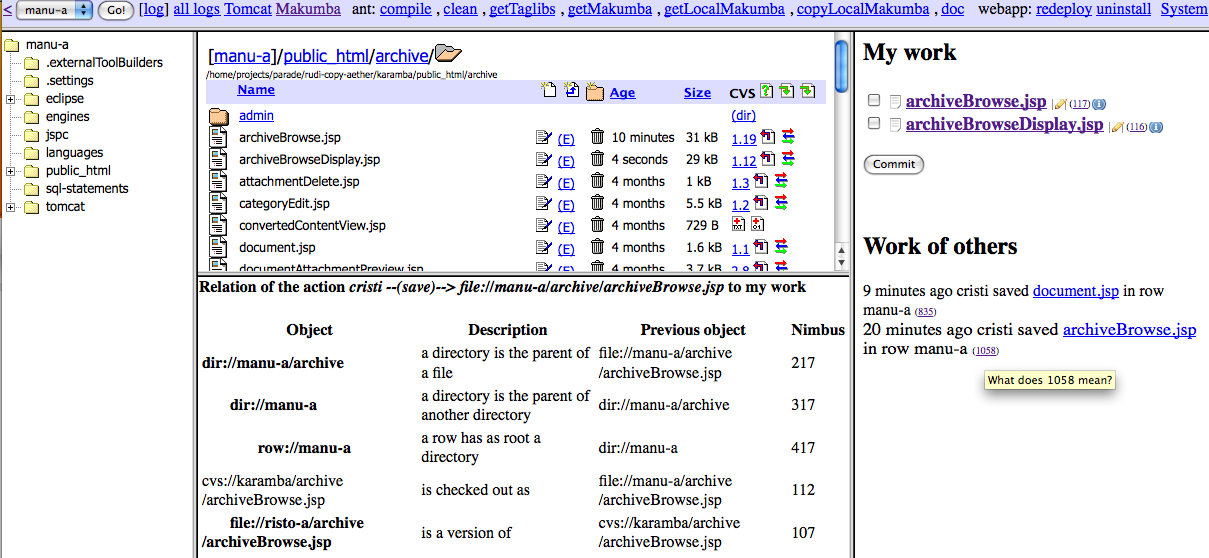
\includegraphics[width=.98\linewidth]{nimbus-history}
  \caption{ParaDe: initial interface (top, centre, left), on which we added the initial awareness widgets (right) and percolation explanation (bottom). These 'awareness engine' frames were enlarged for illustration purposes}
  \label{fig:parade}
\end{figure}

\section*{Awareness engine implementation} 
Besides our AETHER-related concerns already expressed, we aimed to implement an awareness engine that would not make many ParaDe-related assumptions and that would be usable without compromising the present user experience, in terms of e.g. response time and familiarity with the present interface. Based on earlier experiences with AETHER described by \cite{sandor97} we identified \textit{performance of percolation} as an important design constraint for our architecture. In order to be able to process a large semantic network such as ParaDe's in satisfactory time, we decided to employ database management system (DBMS) technologies, which are designed to perform well for large amounts of data. In the DBMS domain, the \textit{database query} is a fundamental unit of work, and is typically written in a variant of Structured Query Language (SQL). While DBMS systems are optimized to run most queries fast enough, the single most important performance factor of an application (e.g.  ParaDe or the awareness engine) employing a DBMS is the number of queries sent from the application to the DBMS. As part of our work with another technology (Makumba, www.makumba.org) we acquired quite a lot of experience with \textit{query-centric} ways of developing applications, especially in regard to aggregating more \textit{query fragments} into a single query, to reduce the number of queries sent to the database back-end (DBMS).  We decided to apply such query aggregation techniques here,  and thus we have obtained a query-centric awareness engine implementation. 

\subsection*{Building the semantic network}
The data that the awareness engine primarily works with is the ParaDe data, which models applications (like the Intranet) and copies of the application. Each application copy contains a large set of files. A user (the copy owner) is also associated to the application copy. Over this data, a semantic network is created by defining relations among these objects. Some relations are stored in the database explicitly, like the relation between an application copy and the owner, or the code dependency relation between two files. However, we chose to define many of our relations using \textit{relation rules}, which are stored by the awareness engine as query fragments. As such, we chose not to represent some relations in the database explicitly, but to generate relations when we need them (during percolation) by integrating their query fragments in the queries we run for percolation. The reason for this is that the number of objects stored in the database would multiply manyfold if we would explicitly represent relations such as "file is in directory" or "file isVersionOf  repositoryFile", and this would affect performance and would make the semantic network more difficult to maintain. Instead, both exemplified relations are determined based on the file path. Another reason is that using relation rules allows us to create an awareness engine over any existing database. For uniformity, even the relations that are represented explicitly in our database are retrieved through relation rules. The rules become \textit{data} for the awareness engine, and the query fragments are actually stored in the database and can be changed at awareness engine runtime. Below we exemplify a relation rule that defines a \texttt{parentOf} relation between a  file and its containing directory. 

\begin{quote}\texttt{SELECT f.parentURI() as toURI, 'parentOf' as type, f.URI() as fromURI \\*
FROM File f \\*
WHERE f.URI() IN(:fromURISet)}
\end{quote}

The rule query is used as a fragment, i.e. its sections (FROM, WHERE) can be combined with sections from other queries during percolation. The query parameter \texttt{:fromURISet} is a value maintained during the percolation process. The functions \texttt{parentURI()} and \texttt{URI()} are expanded by the Makumba technology in the queries sent to the DBMS. Their implementation, defined in relation to the \texttt{File} data type is essentially made of a series of string processing SQL calls. For example \texttt{parentURI()}, given \texttt{file://a/b.txt} returns \texttt{dir://a} by processing the URI strings. Using such functions allows us to simplify a lot the query fragments employed by the awareness engine for defining rules. 

\subsection*{Percolation}
Once the semantic network is defined (in a dynamic way via relation rules), we have the space over which we can percolate. Firstly, we maintain an action log, which collects all user actions such as opening a directory, compiling an application, looking at a file, changing a file, deploying an application for execution in a web application engine, accessing the web page produced by a source code file, etc. This action log will be application dependent, however, the only assumption made by our awareness engine implementation is that the action log is represented in the database, which is not uncommon for current logging systems. Once the actions are registered in the database, we can define \textit{initial percolation rules} to trigger percolation based on some action logged. Like relation rules, initial percolation rules can be changed at engine runtime, new rules can be added, and existing ones can be de-activated. The following example illustrates an initial percolation rule for percolating nimbus on file save:
\begin{quote}objectType:\texttt{FILE}\\*
action: \texttt{save}\\*
userType: \texttt{all\_but\_actor}\\*
initialLevel: \texttt{100}\\*
percolationMode: Nimbus\\*
interactionType	: Deferred \\*
active: Yes\\*
relation rules to follow: \texttt{parentOf}, \texttt{dependsOn}, \texttt{versionOf} \\*
nimbus progression curve: \texttt{1-t*t+t} \\*
\end{quote}

This initial percolation rule will match actions of type 'save' on objects of type FILE. They will begin nimbus percolation towards any other user than the user who produced the action (\texttt{all\_but\_actor}), with an initial strength of 100. The strength will vary in time according to a given progression curve, so  the event "loses in importance" as time goes by (this however can be compensated by large focus value for a certain user). The first percolation step will start over relations of type \texttt{parentOf} (exemplified above), \texttt{dependsOn} (source file dependency) and \texttt{versionOf} (relations to the reference file versions in the CVS repository).

Once percolation has reached a new set of objects via such initial relations, \textit{percolation rules} apply. Once a certain kind of relation has been traversed, a percolation rule defines what types of relations to look for next, and how much to consume from the existing focus or nimbus strength. For example the following rule specifies a consumption of 20 units on each file dependency percolation, and specifies to take next either a dependency relation or a version relation. The "description" of the rule can be used to generate a textual description of a percolation path, for example to explain to a user why they were notified of a certain event. A prototype version of such an explanation is shown at the lower part of Figure \ref{fig:parade}. Such explanation of complex internal mechanisms is addressing our \textit{translucency concern}. Users can examine and possibly alter the rules that applied during a percolation, which addresses our \textit{tailoring concern}.

\begin{quote}
subject: \texttt{FILE}\\*
predicate: \texttt{dependsOn}\\*
object:\texttt{FILE}\\*
consumption: 20\\*
description: depends on the file that was acted upon\\*
active: Yes\\*
relation rules to follow: \texttt{dependsOn}, \texttt{versionOf} \\*
\end{quote}
For every relation rule traversal (starting with an initial percolation rule or continuing on a percolation rule), a \textit{percolation step} is saved. By summing up all percolation steps on a certain object for a certain user (or user group) we obtain the total focus and nimbus levels for that user and object, which allows us to compute the awareness level. Summing up allows us to account for arriving at an object through multiple paths during percolation, or to sum "old" percolations which still have some initial strengths as per their time progression curve with "new" (more recent) event percolations, i.e.  we accumulate focus or nimbus levels both \textit{spatially} and \textit{temporally}. Percolation steps where the focus and nimbus levels "dies out" according to the progression curves are cleaned from the database, thereby resulting in a manageable number of objects and sustainable use of database storage space. Registering percolation steps also allows us to explain to users how a percolation took place, as already mentioned.  

\subsection*{User interface and Plan for experimentation}
Addressing our \textit{focus-nimbus manipulation concern} is the most challenging part of our awareness engine work, and we plan to continue this during our experimentation, together with the ParaDe users. For starters, we designed two  'widgets' called "my work" and "work of others". "My work" (Figure \ref{fig:parade} top right) shows the actions of the user from which successful focus percolation took place. The user focus is thus initially built from the objects they have worked with. Out of these, the modification actions can also be committed to the CVS repository, thereby bringing added value to the "my work" widget. To add other objects to their focus, the will be able to click on a "watch" widget near that object. To increase the nimbus of one of their actions, the user will be able to use a "show" widget.

The "work of others" widget  (Figure \ref{fig:parade} lower right)  shows objects that had a focus-nimbus match and thus have a certain awareness level at the moment. In this prototype version of the widget, the size of the text in work of others is dependent on the awareness level, which is also explicitly shown. By clicking on the "work of others" information, the user can obtain the percolation explanation depicted at the bottom of Figure \ref{fig:parade}.

%virtual percolation

%the community feeling, relaxed focus

%anticipative awareness

\section*{Conclusion}
We could metaphorically say that ParaDe is for awareness engine experimentation what an "ideal gas" is for thermodynamics. While it is difficult to find nowadays real-world work arrangements where a semantic network can be built with such completeness and accuracy, we believe that for example Semantic Web technologies can advance this field so that also non-programming activities and more heterogeneous and distributed systems will in the future benefit from a better-quality semantic network. In the meantime, our experiments with the "ideal gas" in the ParaDe programming domain can help us find principles and practices that will be useful for other types of collaborative distributed work.

%\begin{figure}[thb]
%  \centering
%  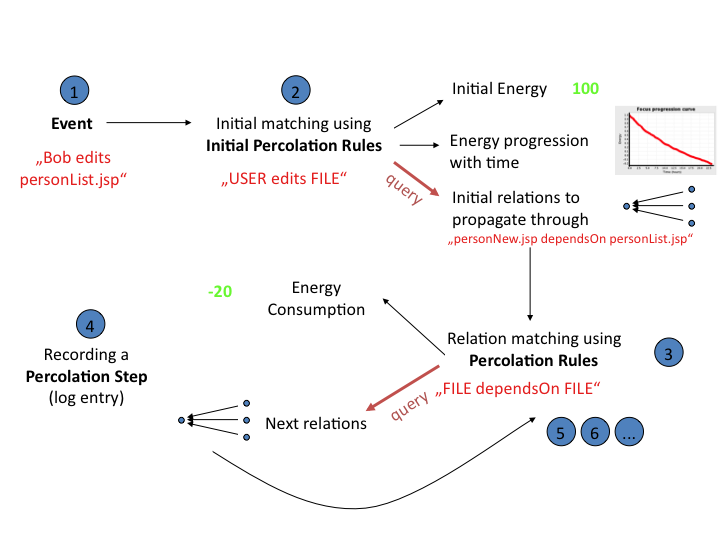
\includegraphics[width=.7\linewidth]{aether-mechanism}
%  \caption{Aether mechanism}
%  \label{fig:aether-mechanism}
%\end{figure}

\bibliography{ecscw09-aether}
\bibliographystyle{ecscw2007}  

\end{document}

% Local Variables:
% TeX-master: t
% End:
